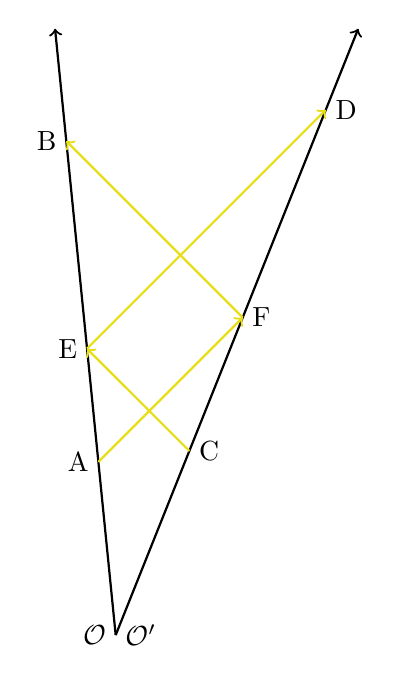
\begin{tikzpicture}[scale=1.1]
	% Draw lines of observers
	\draw[->, thick] (-0.6, -4) -- (-1.3, 3);
	\draw[->, thick] (-0.6000000000000001, -4) -- (2.2, 3);
	
	% Draw trajectories of light
	\draw[->, thick, black!10!yellow] (-0.8, -2) -- (0.8666666666666667, -0.33333333333333326);
	\draw[->, thick, black!10!yellow] (0.8666666666666667, -0.33333333333333326) -- (-1.1703703703703705, 1.703703703703704);
	\draw[->, thick, black!10!yellow] (0.2504201680672269, -1.8739495798319328) -- (-0.930718954248366, -0.6928104575163399);
	\draw[->, thick, black!10!yellow] (-0.930718954248366, -0.6928104575163399) -- (1.8252723311546843, 2.0631808278867103);
	
	% Make labels
	\draw (-0.6, -4) node[left] {$\mathcal{O}$};
	\draw (-0.8, -2) node[left] {A};
	\draw (-1.1703703703703705, 1.703703703703704) node[left] {B};
	\draw (0.8666666666666667, -0.33333333333333326) node[right] {F};
	\draw (-0.6000000000000001, -4) node[right] {$\mathcal{O}'$};
	\draw (0.2504201680672269, -1.8739495798319328) node[right] {C};
	\draw (1.8252723311546841, 2.0631808278867103) node[right] {D};
	\draw (-0.930718954248366, -0.6928104575163399) node[left] {E};
\end{tikzpicture}